\section{Main Figures}

\subsection{Figure 1}

\begin{figure*}[H]
\refstepcounter{figure}\label{fig:workflow_graphic}
\centering
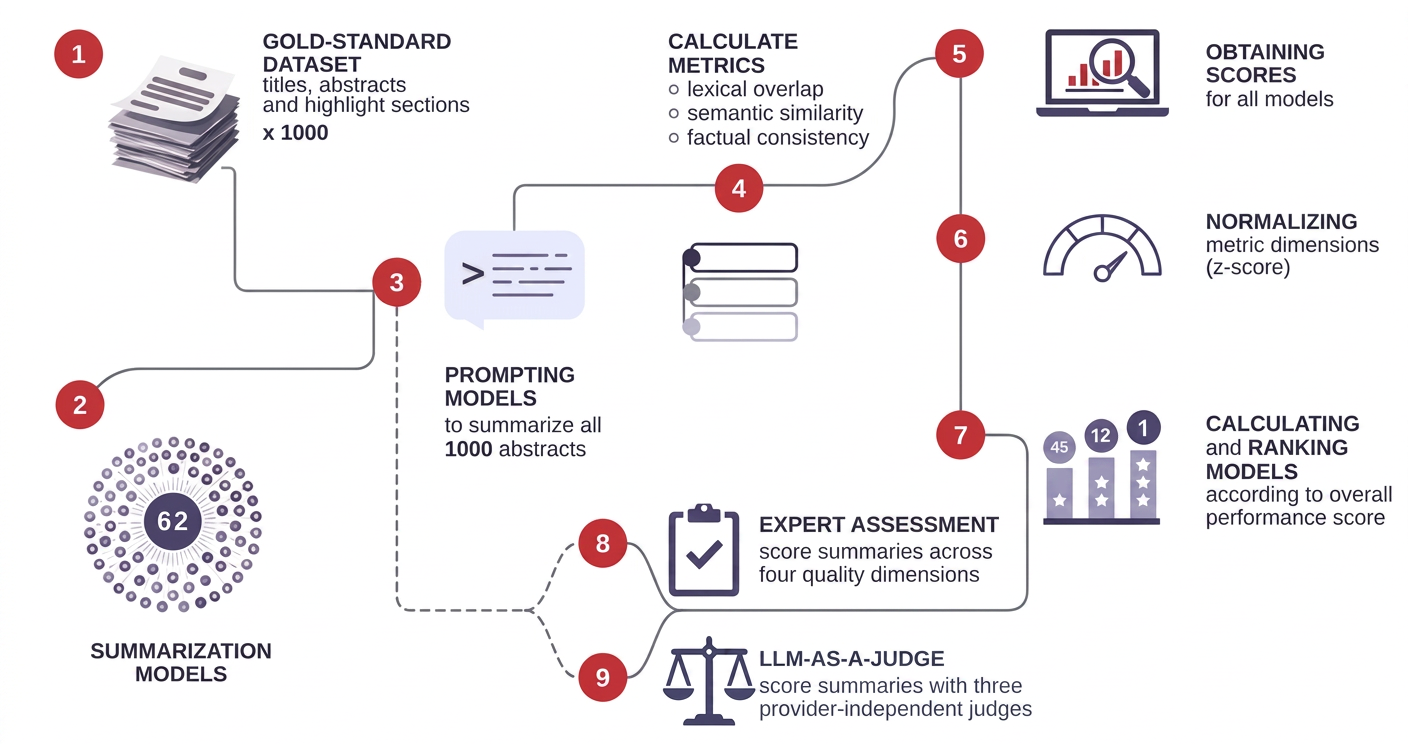
\includegraphics[width=0.9\textwidth]{Visualizations/workflow_graphic_9steps_polished.png}
\end{figure*}

\subsection{Figure 2}

\begin{figure*}[H]
\refstepcounter{figure}\label{fig:metric_correlation}
\centering

\includegraphics[width=0.85\textwidth]{Visualizations/metric_correlation.png}
\end{figure*}

\subsection{Figure 3}

\begin{figure*}[H]
\refstepcounter{figure}\label{fig:rank_heatmap}
\centering

\includegraphics[width=0.7\textwidth]{Visualizations/rank_heatmap.png}
\end{figure*}

\subsection{Figure 4}

\begin{figure*}[H]
\refstepcounter{figure}\label{fig:category_boxplots_and_gameshowell}
\centering

\includegraphics[width=0.85\textwidth]{Visualizations/category_boxplot.png}
\vspace{8pt}

\includegraphics[width=0.85\textwidth]{Visualizations/category_gameshowell.png}
\end{figure*}

\subsection{Figure 5}

\begin{figure*}[H]
\refstepcounter{figure}\label{fig:family_boxplots_and_gameshowell}
\centering

\includegraphics[width=0.85\textwidth]{Visualizations/family_boxplot.png}
\vspace{8pt}

\includegraphics[width=0.85\textwidth]{Visualizations/family_gameshowell.png}
\end{figure*}

\subsection{Figure 6}

\begin{figure*}[H]
\refstepcounter{figure}\label{fig:assessment_results}
\centering
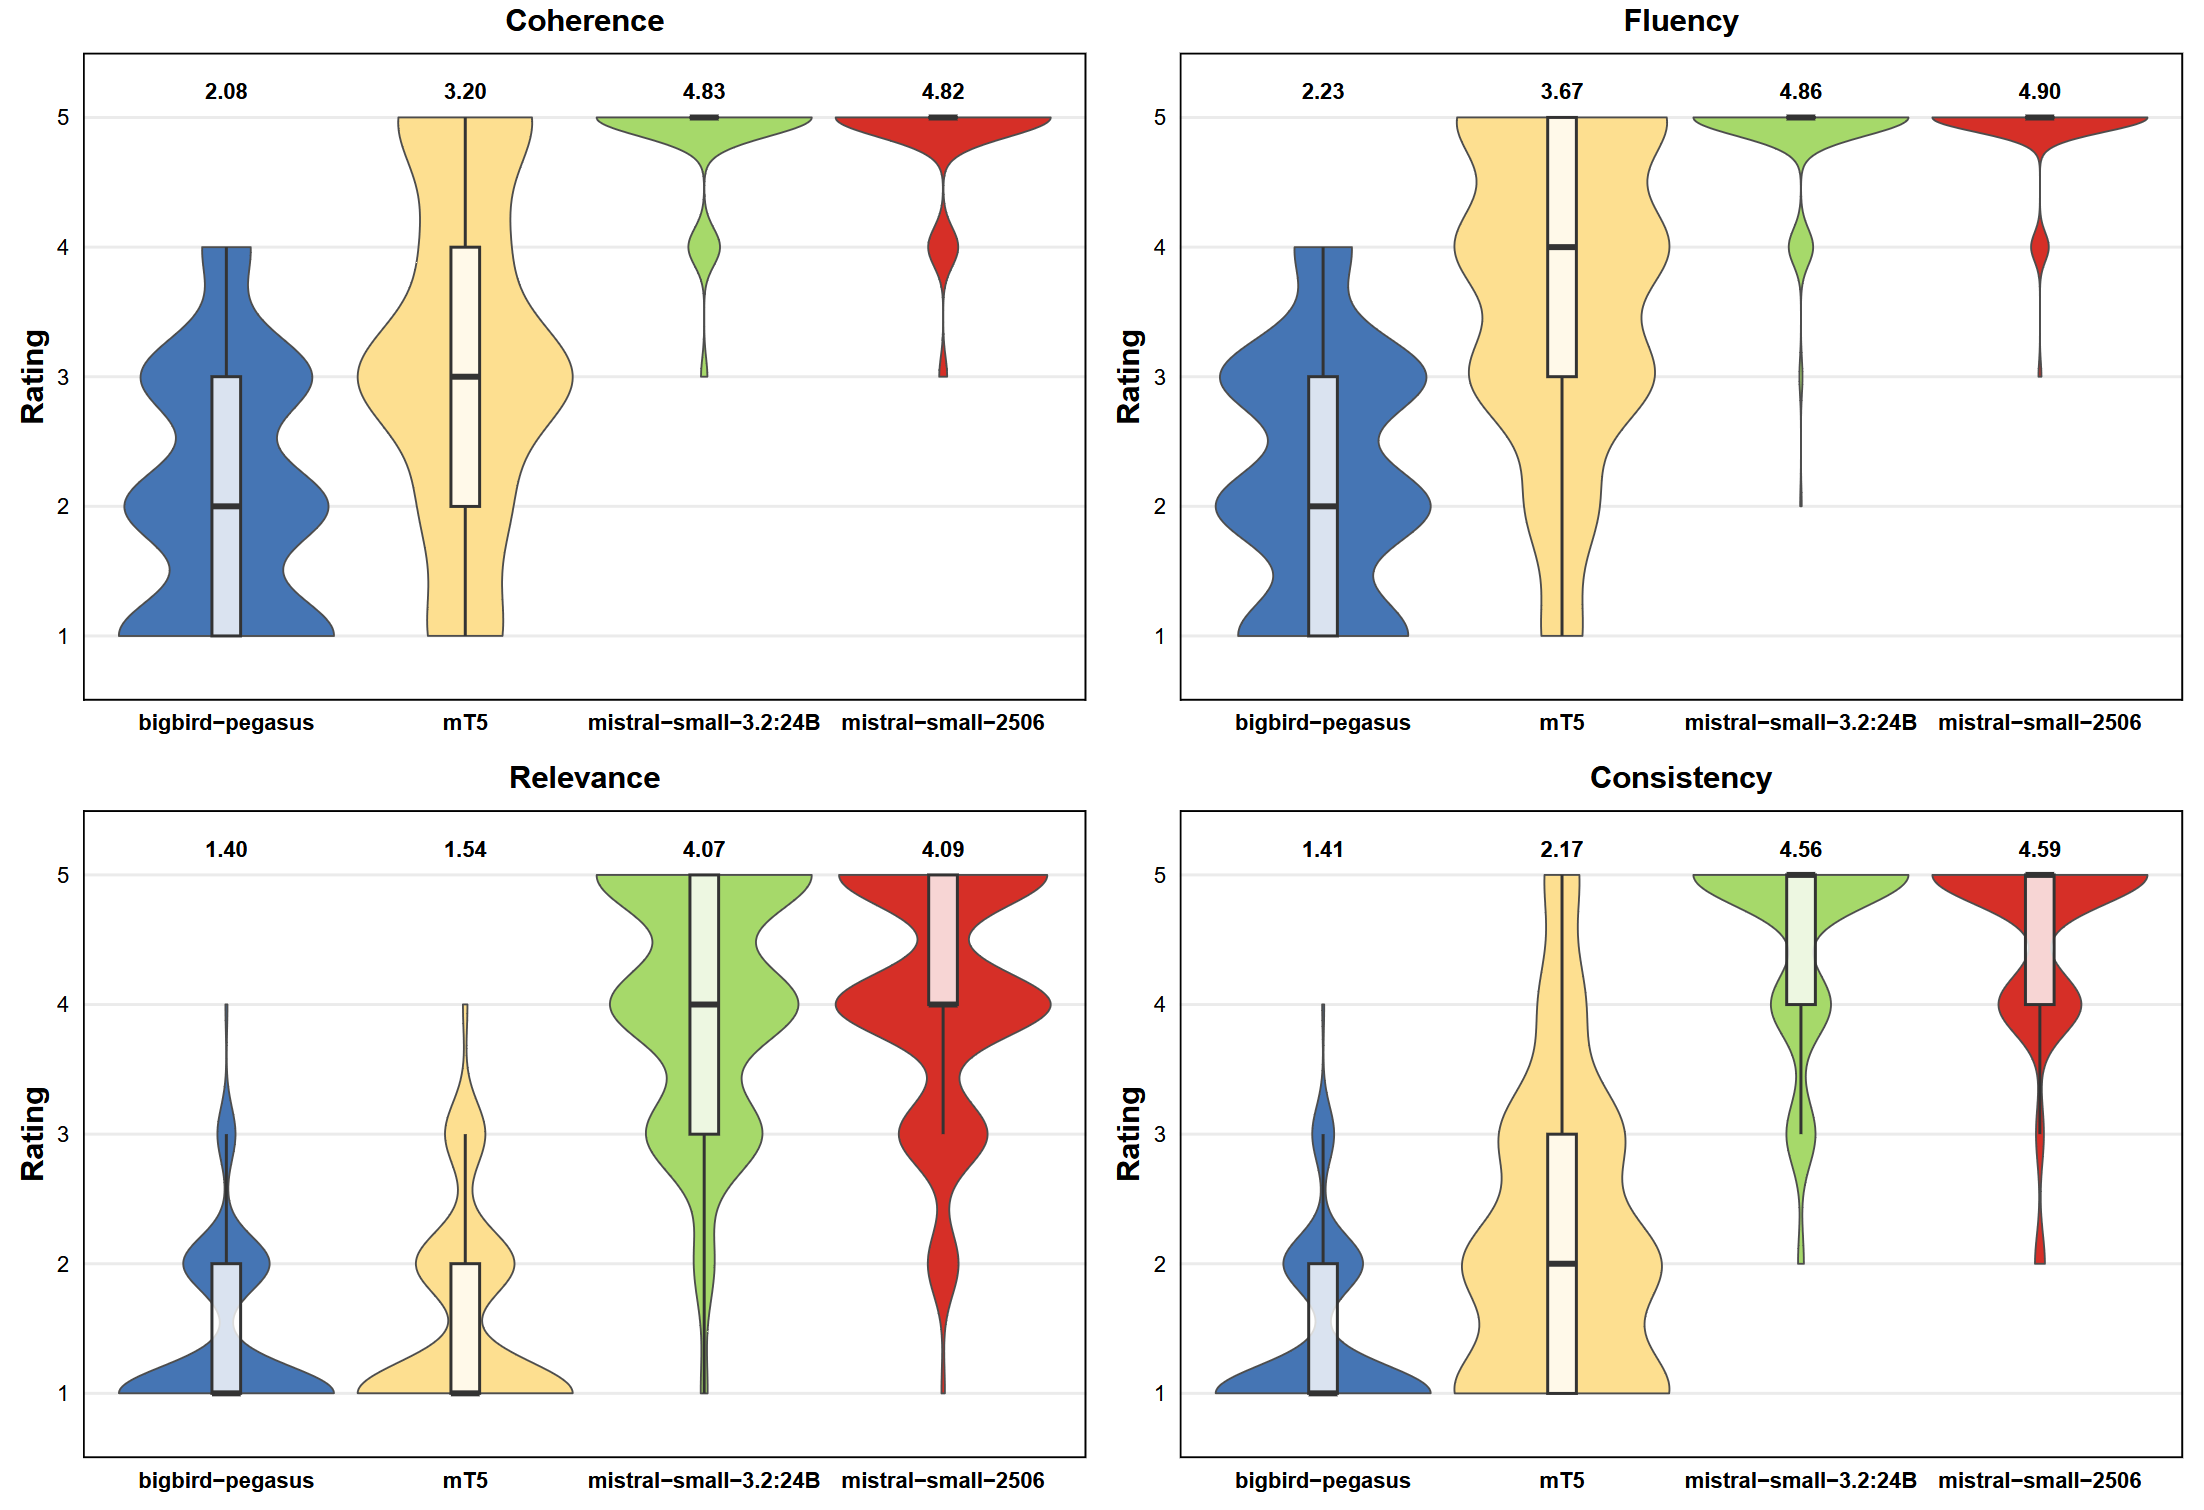
\includegraphics[width=0.95\textwidth]{Visualizations/assessment_results.png}
\end{figure*}

\subsection{Figure Legends}

\begin{itemize}
	\item Figure 1: \textbf{Overview of the benchmarking workflow:} (1) Construction of a gold-standard dataset comprising 1,000 biomedical titles, abstracts, and author-provided highlight sections. (2) Suite of 62 diverse summarization models. (3) Uniform prompting of all models to generate summaries for each abstract. (4--5) Computation of summary quality metrics capturing lexical overlap, semantic similarity, and factual consistency. (6) Standardization of metric scores using z-score normalization to ensure comparability across evaluation dimensions. (7) Ranking of models based on overall performance scores. (8) Quality assessment of generated summaries across four quality dimensions (coherence, fluency, relevance, consistency), combining expert human evaluation on a subset of models with (9) \ac{LLM}-as-a-judge evaluation from three provider-independent judges run across all models.
	\item Figure 2: \textbf{Spearman correlation between evaluation metrics:} Spearman correlation coefficients ($\rho$) between two metrics based on their mean scores across all models are given. Metric categories (lexical, semantic, factual) are indicated on the x and y axes. For visualization purposes, cells with values higher than 0.8 are shown with white text.
	\item Figure 3: \textbf{Ranking of summarization models:} Overview of the performance of all evaluated models across lexical, semantic, and factual metric dimensions. Each row corresponds to one model. Columns show the overall Performance Rank and independent ranks for each metric dimension, with lower ranks indicating better performance. The figure displays each model’s family and category. Models are sorted by the overall Performance Rank. Ranks are displayed using a continuous diverging color gradient, ranging from navy-blue tones for top-performing models through light neutral shades for mid-ranked models to dark red tones for low-performing models. 
	\item Figure 4: \textbf{(a) Overall performance of model categories:} Distributions of overall performance scores across the nine model categories, with each model represented by a black dot. Categories are ordered from lowest to highest-performing according to the median performance score. The best- and worst-performing models of each category are highlighted. \textbf{(b) Games-Howell Post-hoc Test across model categories:} Games-Howell pairwise adjusted $p$-value matrix comparing all category pairs. Each cell shows the adjusted $p$-value for the difference in metric mean scores between two categories, with white-to-gray shading indicating smaller $p$-values.
	\item Figure 5: \textbf{(a) Overall performance of model families:} Distributions of overall performance scores across all model families, with each model represented by a black dot. Families are ordered from lowest to highest-performing according to the performance score. The best- and worst-performing models of each family are highlighted. \textbf{(b) Games-Howell Post-hoc Test across model families:} Games-Howell pairwise adjusted $p$-value matrix comparing all family pairs. Each cell shows the adjusted $p$-value for the difference in metric mean scores between two families, with white-to-gray shading indicating smaller $p$-values.
	\item Figure 6: \textbf{Expert assessment results across four quality dimensions:} Distribution of expert ratings for coherence, fluency, relevance, and consistency for each model are shown with average ratings shown above the box-violin plots.
	


\end{itemize}